\documentclass{ijsra}
\def\IJSRAidentifier{\currfilebase} %<---- don’t change this!
\def\submission{}%YYYY-MM-DD
\def\acceptance{}%YYYY-MM-DD
%-------Title | Email | Keywords | Abstract-------------
\def\shorttitle{Ship-Themed Scandinavian Burials}
\def\maintitle{There and Back Again: Ancestor Veneration and Necromancy in Ship-Themed Scandinavian Burials}
\def\cmail{Cassandra.clark@ucdconnect.ie}
\def\keywords{ship, burial, Scandinavia, Viking, necromancy, ancestor worship, picture stone}
%\def\keywordname{}%<--- redefine the name “Keywords“ in needed language
\def\abstract{Many interpretations have been applied to ship symbolism in Scandinavian mortuary contexts, the most common of which describes the ship as a vessel to transport the dead from one world to the next. However, many of these interpretations fail to address the role of the ship in the context of cultic practices described in contemporary literature. Through an assessment of literary sources and archaeological evidence present in ship burials, stone ship settings, and picture stones, this paper aims to address these interpretive gaps, making a case for ancestral referencing and veneration as well as necromantic ritual in ship-themed burials. I do not attempt to disentangle ship symbolism from the concept of travel, but rather argue that mortuary ships allow the dead the freedom to depart from and return to the world of the living.}
%--------Author’s names------------
\def\authorone{Cassandra Clark}
%-------Biographical information-------------
\def\bioone{Cassandra Clark is an American archaeologist specialising in the archaeological studies of death, gender, and shamanic and pre-Christian beliefs and practices. She earned her BA in Art History from University of Nebraska-Omaha in 2016, where she wrote her undergraduate thesis on the influence of rock art and architecture upon mortuary and ancestral ritual in Irish Neolithic passage tombs. Clark then moved to Ireland to complete her master’s degree in archaeology at University College Dublin. It was there that she developed her passion for studying the intersection between gender and the materiality of shamanism in mortuary settings. Utilizing burials of female shamans from pre-Columbian North, South, and Central America, she wrote her master’s thesis on the gendered expression of shamanism in funerary contexts. Clark graduated from University College Dublin in December 2017, and presented the results of her master’s thesis at an international conference in Vietnam that same month. She aims to begin a PhD program in the next several years, at which time she intends to study the origins and material expressions of shamanism and sorcery in medieval Europe.}
%------University/Institution--------------
\def\affilone{University College Dublin}

\begin{filecontents}{\IJSRAidentifier.bib}
@Article{Ballard_2004,
	author    = {Ballard, Chris and Bradley, Richard and Myhre, Lise Nordenborg and Wilson, Meredith},
	title     = {The ship as symbol in the prehistory of Scandinavia and Southeast Asia},
	journal   = {World Archaeology},
	year      = {2004},
	volume    = {35},
	number    = {3},
	pages     = {385--403},
	publisher = {Taylor \& Francis},
}

@Article{Bill_2016,
	author  = {Bill, Jan},
	title   = {Ambiguous Mobility in the Viking Age Ship Burial from Oseberg},
	editor = {I Peter Bjerregaard and Anders Emil Rasmussen and Tim flohr S{\o}rensen},
	booktitle = {Materialities of Passing: Explorations in Transformation, Transition and Transience},
	year    = {2016},
	pages   = {207--220},
}

@Article{Bradley_2010,
	author  = {Bradley, Richard and Skoglund, Peter and Wehlin, Joakim},
	title   = {Imaginary vessels in the Late Bronze Age of Gotland and South Scandinavia},
	journal = {Current Swedish Archaeology},
	year    = {2010},
	volume  = {18},
	pages   = {79--103},
}

@Article{Price_2008,
	author    = {Price, Neil},
	title     = {Dying and the dead: Viking Age mortuary behaviour},
	journal   = {The Viking World},
	year      = {2008},
	pages     = {257--73},
	publisher = {Routledge London},
}

@MastersThesis{Wehlin_2010,
	author    = {Wehlin, Joakim},
	title     = {Approaching the Gotlandic Bronze Age from sea: future possibilities from a maritime perspective},
	school    = {University of Gothenbourg/Gotland University},
	year      = {2010},
	publisher = {Gotland university},
}

@Article{Williams_2010,
	author    = {Williams, Howard and Rundkvist, Martin and Danielsson, Arne},
	title     = {The landscape of a Swedish boat-grave cemetery},
	journal   = {Landscapes},
	year      = {2010},
	volume    = {11},
	number    = {1},
	pages     = {1--24},
	publisher = {Taylor \& Francis},
}

@Article{Skoglund_2008,
	author    = {Skoglund, Peter},
	title     = {Stone ships: continuity and change in Scandinavian prehistory},
	journal   = {World Archaeology},
	year      = {2008},
	volume    = {40},
	number    = {3},
	pages     = {390--406},
	publisher = {Taylor \& Francis},
}

@Article{Hansson_1998,
	author  = {Hansson, Martin},
	title   = {Graves, Grave-Fields and Burial Customs},
	journal = {Lund Archaeological Review for 1998},
	year    = {1998},
	pages   = {49--65},
}

@Book{Herschend_2001,
	title     = {Journey of Civilization: The Late Iron Age View of the Human World},
	publisher = {(Uppsala, Uppsala University Department of Archaeology and Ancient History)},
	year      = {2001},
	author    = {Herschend, F},
}

@Article{Rundkvist_2008,
	author    = {Rundkvist, Martin and Williams, Howard},
	title     = {A Viking boat grave with amber gaming pieces excavated at Skamby, {\"O}sterg{\"o}tland, Sweden},
	journal   = {Medieval Archaeology},
	year      = {2008},
	volume    = {52},
	number    = {1},
	pages     = {69--102},
	publisher = {Taylor \& Francis},
}

@incollection{Sanmark_2010,
	author  = {Sanmark, Alexandra},
	title   = {Living on: Ancestors and the soul},
	booktitle = {Signals of Belief: Anglo-Saxon Paganism Revisited},
	year    = {2010},
	pages   = {162--184},
}

@Article{Sundqvist_2015,
	author  = {Sundqvist, Olof},
	title   = {The Pre-Christian Cult of Dead Royalty in Old Norse Sources: Medieval Speculations or Ancient Traditions?},
	journal = {Scripta Islandica: Isl{\"a}ndska S{\"a}llskapets {\AA}rsbok},
	year    = {2015},
	volume  = {66},
	pages   = {177--212},
}

@Article{Nordberg_2013,
	author  = {Nordberg, A.},
	title   = {Fornnordisk religionsforskning mellan teori och empiri},
	journal = {Acta Academiae regiae Gustavi Adolphi},
	year    = {2013},
	volume  = {CXXVI},
}

@Book{Price_2015,
	title     = {Ancient Scandinavia: An archaeological history from the first humans to the Vikings},
	publisher = {Oxford University Press, USA},
	year      = {2015},
	author    = {Price, Theron Douglas},
}

@MastersThesis{Gustavsson_2012,
	author = {Gustavsson, Anders},
	title  = {Artefacts and bone patterns in stone ship settings on Gotland},
	school = {University of Gotland},
	year   = {2012},
}

@Electronic{Price_2012a,
	author       = {Neil Price},
	title        = {The Shape of the Soul: The Viking Mind and the Individual},
	organization = {youtube},
	url          = {https://www.youtube.com/watch?v=7Db9sG1PSsQ&t=1169s},
	date         = {2012},
}

@Electronic{Price_2012b,
	author       = {Neil Price},
	title        = {Life and Afterlife: Dealing with the Dead in the Viking Age},
	organization = {youtube},
	url          = {https://www.youtube.com/watch?v=uu2gN8n15_A&t=1694s},
	date         = {2012},
}

@MastersThesis{Ruffoni_2011,
	author = {Ruffoni, Kirsten},
	title  = {Viking Age Queens: The example of Oseberg},
	school = {University of Oslo},
	year   = {2011},
}

@Article{Runesson_2010,
	author  = {Runesson, Gunilla},
	title   = {Gotlandic Bronze Age Settlements in Focus},
	journal = {Baltic Prehistoric Interactions and Transformations},
	year    = {2010},
	pages   = {79},
}

@Article{Eriksen_2013,
	author    = {Eriksen, Marianne Hem},
	title     = {Doors to the dead. The power of doorways and thresholds in Viking Age Scandinavia},
	journal   = {Archaeological dialogues},
	year      = {2013},
	volume    = {20},
	number    = {2},
	pages     = {187--214},
	publisher = {Cambridge University Press},
}

@Article{Montgomery_2000,
	author  = {Montgomery, James E},
	title   = {Ibn Fadlan and the R{\=u}siyyah},
	journal = {Journal of Arabic and Islamic studies},
	year    = {2000},
	volume  = {3},
	pages   = {1--25},
}

@Article{Wallin_2010,
	author  = {Wallin, Paul},
	title   = {Neolithic monuments on Gotland: material expressions of the domestication process},
	journal = {Baltic Prehistoric Interactions and Transformations: The Neolithic to the Bronze Age},
	year    = {2010},
	pages   = {39--62},
}

@Article{Helskog_1999,
	author    = {Helskog, Knut},
	title     = {The shore connection. Cognitive landscape and communication with rock carvings in northernmost Europe},
	journal   = {Norwegian archaeological review},
	year      = {1999},
	volume    = {32},
	number    = {2},
	pages     = {73--94},
	publisher = {Taylor \& Francis},
}

@Article{Westerdahl_2005,
	author    = {Westerdahl, Christer},
	title     = {Maritime cosmology and archaeology},
	journal   = {Deutsches Schiffahrtsarchiv},
	year      = {2005},
	volume    = {28},
	pages     = {7--54},
	publisher = {DEU},
}

@Article{Westerdahl_2015,
	author    = {Westerdahl, Christer},
	title     = {The Viking Ship in Your Mind. Some comments on its cognitive roles},
	journal   = {Årbok Norsk Maritimt Museum},
	year      = {2015},
	volume    = {14},
	pages     = {33-70},
	publisher = {Årbok Norsk Maritimt Museum},
}

@Article{Artursson_2013,
	author  = {Artursson, Magnus},
	title   = {SHIPS IN STONE: SHIP-LIKE STONE SETTINGS, WAR CANOES AND SAILING SHIPS IN BRONZE AGE SOUTHERN SCANDINAVIA},
	journal = {Counterpoint: Essays in Archaeology and Heritage Studies in Honour of Professor Kristian Kristiansen},
	year    = {2013},
	pages   = {499--504},
}

@Article{Skoglund_2009,
	author    = {Skoglund, Peter},
	title     = {Beyond chiefs and networks: corporate strategies in Bronze Age Scandinavia},
	journal   = {Journal of Social Archaeology},
	year      = {2009},
	volume    = {9},
	number    = {2},
	pages     = {200--219},
	publisher = {SAGE Publications Sage UK: London, England},
}

@InBook{Skoglund_2014,
	pages     = {201-214},
	title     = {Social landscapes of Bronze Age Scandinavia},
	publisher = {Routledge},
	year      = {2014},
	author    = {Skoglund, Peter},
	journal   = {Local Societies in Bronze Age Northern Europe},
}

@Book{Kaul_1998,
	title     = {Ships on Bronzes: A Study in Bronze Age Religion and Iconography: Catalogue of Danish Finds. II},
	publisher = {National Museum of Denmark, Department of Danish Collections},
	year      = {1998},
	author    = {Kaul, Flemming},
}

@Article{Manguin_1986,
	author    = {Manguin, Pierre-Yves},
	title     = {Shipshape societies: boat symbolism and political systems in insular Southeast Asia},
	journal   = {Southeast Asia in the 9th to 14th Centuries},
	year      = {1986},
	pages     = {187--213},
	publisher = {Singapore: ISEAS \& Canberra: ANU},
}

@Comment{jabref-meta: databaseType:bibtex;}

\end{filecontents}
\IJSRAopening%<---- don’t change this!
%-------
\lettrine{T}{he} symbolism of the ship or boat in Scandinavian mortuary contexts has long been a topic of debate. With an expansive history stretching from the Mesolithic into the late Viking Age, there can be no doubt that the symbol acquired a great multiplicity of meanings over time. It is arguably the most prolific motif of this culture, and is found depicted on rock art and bronze artifacts from central to south Scandinavia, on stone ship settings in mainland Sweden and the island of Gotland, in ship burials both in Scandinavia and abroad, and upon the massive and intricately decorated Gotlandic picture stones \parencites[264--266]{Price_2008}[93]{Wehlin_2010}. While it is not difficult to understand why ships would be greatly revered as a symbol in a maritime economy such as this, the reasoning for the relationship between ships and the afterlife in early Scandinavia remains a matter of speculation.

Interpretations regarding the significance of mortuary ship symbolism during Scandinavia’s Bronze, Iron, Pre-Viking and Viking Ages have been plentiful and varied. Some argue that these objects and symbols stood as metaphors not only for an individual’s position within his or her community, but also for the relationship between Scandinavia and Continental Europe \parencite[388]{Ballard_2004}.
Indeed, ships were not only metaphors for travel and trade; some ship burials bore markers of the identity, ethnicity, religious ideologies, and power of the individual interred within them \parencite[265]{Price_2008}.
Other scholars theorize that ship burials and megalithic monuments constructed in the form of ships (hereafter referred to as stone ship settings) were intentionally built near the sea as navigation aids for travelers and traders \parencite[388]{Ballard_2004}.
Interpretive distinctions have also been made regarding the ship’s underlying meaning particular to time period and the medium used to craft these mortuary vessels. Bronze and Iron Age stone ship settings have variously been interpreted as embodiments of communal or familial identity \parencite[390]{Ballard_2004}
, great symbolic warships \parencite[394--396]{Skoglund_2008},
and as cult houses where ancestral ritual may have taken place \parencite[97]{Bradley_2010}. Burials containing actual ships are understood by many scholars either in the context of their use in transportation (specifically, in transporting the dead to some version of the afterlife) or as a show of wealth and grandeur by the deceased and their families \parencite[265]{Price_2008}.
Picture stones, which occur almost exclusively on the island of Gotland, are generally perceived as continuations of the connection between ships and the afterlife, since the bottom register of these intricately carved markers nearly always contains a ship \parencite[265]{Price_2008}. These interpretations emphasize the ship’s undeniably crucial role in Scandinavia’s development through the ages. Although the manifestations of afterlife cosmology may at first appear different after considering these analyses, I argue that the underlying beliefs, practices, and interactions with mortuary ships and ship symbols may have been quite similar across time and monument type.


Most often these real and metaphorical vessels are interpreted as a method of transportation for the dead to the hereafter \parencite[265]{Price_2008}.
However, ship symbolism is not altogether common within mortuary contexts. What distinguishes individuals interred in ship-themed graves from those who did not receive such a burial? Scholars have suggested that ship symbolism in mortuary contexts may be indicative of the high status and aristocratic lifestyle of those with whom the symbols are associated \parencites[61]{Hansson_1998}[68]{Herschend_2001}[4]{Williams_2010}.
The ship may also be representative of ‘heroic worldly ordeals \parencite[90]{Rundkvist_2008},” possibly elevating the identity of the deceased individual to heroic or deified status. If this is the case, perhaps these were special, powerful people – men, women, and families – who were chosen due to their high status or esteem within the community to act as guardian spirits over the land and the people. This may suggest that ship symbolism in itself may have been an embodiment of ancestor veneration and hero cult practice.

Based upon evidence from picture stones, stone ship settings, and ship burials, I hypothesize that ship-themed graves, like other burial monuments, were a loci of interaction between the living and the dead. The following two sections address the ways in which references to lineage and ancestor worship can be discerned from all types of ship-related burials. I do not attempt to dispel or disentangle the association between ships and travel, even in funerary contexts; rather the opposite. Secular interpretations of ship symbolism emphasize the ship’s use in exploring, raiding, trading, expanding, and ultimately returning home; clearly, these vessels were not built to be used only once. It is therefore not far-fetched to consider that these mortuary ships, too, were capable of making more than one journey – not only of sailing to the realm of the dead, but also of returning to the land of the living. I submit that ancestors who were buried with ships or ship symbols could be summoned back from the land of the dead to speak with or aid their living descendants, travelling between worlds via the sea, a well-known boundary between the lands of the living and dead. Furthermore, the ship was symbolically representative of a journey for the dead but, in being a permanent fixture of the landscape, allowed the living to continue their relationship with the individual buried within or beside it. I argue that the permanence of these burial monuments as mounds, doors, or containing metaphorical homes also gave the dead a place within the landscape to return to; in this way, their souls could not lose their way or become trapped. Finally, I theorize that the placement of these markers in liminal places such as shorelines or boundaries between properties or landmarks allowed the dead to travel easily between worlds. There are at least two purposes of ancestral ritual evident from literature and archaeological findings: to venerate and honor the dead through feasts and offerings, or to wake the dead in order to solicit help or arcane knowledge \parencite[171]{Sanmark_2010}. Evidence presented within the following two sections will address my hypotheses regarding these functions in the context of ship-themed burials.

\IJSRAsection{Ancestor Veneration in Ship-Themed Mortuary Contexts}

Although ancestor veneration is an infrequently discussed aspect of pre-Christian Scandinavian ritual and religion \parencites{Nordberg_2013}[][but see]{Sundqvist_2015}, it is nonetheless a critical component in understanding Scandinavian cosmological perspectives and mortuary practice.
Old Norse medieval prose suggests that dead pre-Christian rulers of Scandinavia were honored with public veneration, cult ritual, and sacrifice at their gravesite. After death, these high-status individuals may have been regarded as heroes, mythical beings, or even deities \parencite[177]{Sundqvist_2015}.

As an extension of this practice, evidence indicates that burial mounds themselves may have been regarded as sacred sites. This notion is substantiated by medieval laws from both Sweden and Norway, which prohibit “invocation” or other cultic practices from taking place at burial mounds and other sacred places within the natural landscape. These texts suggest that during the medieval period and likely before, funerary monuments served as loci for cultic practices which may have included ancestor veneration \parencite[198--199]{Sundqvist_2015}.
Many tales from Old Norse prose reveal the belief that the dead even continued living within their graves, such as in the story of Gunnar of Hlidarendi from Njals saga, who startles passersby as he sings loudly in his burial mound one night \parencite[261]{Price_2008}. Admittedly, the accuracy of the Old Norse sagas in depicting non-Christian beliefs and practices has been contested by some due to the heavy influence of Christianity in the 13th century. However, the aforementioned contemporary Scandinavian laws condemning these acts would suggest that the afterlife ideology detailed in the Njals saga was no retelling of a mythical pagan past, but was instead based upon a very real collection of rituals and beliefs practiced concurrently with Christianity.

If it is true that other burial monuments were focal points for ancestor rituals and veneration as medieval laws and sagas suggest, I propose that ship-themed burials were not excluded from these practices. Indeed, references to linage and ancestor worship can be discerned from all forms of ship-related burials. However, the ship symbol may have accorded these burials several layers of meaning; unlike those interred in more typical burial monuments who dwelled within the confines of their mounds, those buried in ship-themed burials could come and go as they pleased upon their ships of death. This and other interpretations will be elucidated within the context of each type of ship-themed burial, including stone ship settings, picture stones, and burials containing actual wooden ships.

The mortuary tradition of stone ship settings is colored by a long and motley history. Though these enigmatic megalithic structures are most commonly associated with Bronze Age Gotland (Fig. \ref{fig:Clark_Figure01}),
earlier examples have been found in southwestern Sweden, Denmark, and Norway, and the construction of ship-shaped stone settings continued into the Iron Age \parencite[92]{Wehlin_2010}.
During its vast history, the ship symbol in this megalithic mortuary context embodied a number of ideologies; perhaps most well-known is the relationship between ships and the solar cosmology established in the Bronze Age. Based upon the appearance of the sun in conjunction with boat imagery found on Scandinavian rock art and bronze razors recovered from funerary contexts, \textcite{Kaul_1998} developed an interpretation in which ships, and their crews, ferried the sun across the sky during the day and under the sea at night.
However, some scholars argue that this solar mythology belongs only to a select portion of society, namely the ruling class, and does not accurately represent the beliefs of the community as a whole. Here it is relevant to consider that the ship symbol and its relationship with the dead predates the Bronze Age \parencite[34]{Westerdahl_2005}.
It therefore seems likely that a cosmology regarding the association between ships and death was already established at this time, and that a new or potentially foreign sun-worshipping belief system adopted and adapted it for the purposes of maintaining community solidarity \parencites[212--213]{Skoglund_2009}[41--42]{Westerdahl_2015}.
What this earlier ideology and its associated rituals might have entailed remains unclear; however, we may look to a comparison between Scandinavian and Southeast Asian ship symbolism \parencite{Ballard_2004} for clues. Although these cultures did not interact with one another, an examination of the significance of the ship as a symbol within a maritime economy such as those found within Southeast Asia may shed light on the mystifying phenomenon of ship-related mortuary practices in Scandinavia’s past.

%FIG 1
\begin{figure}[!htb]
	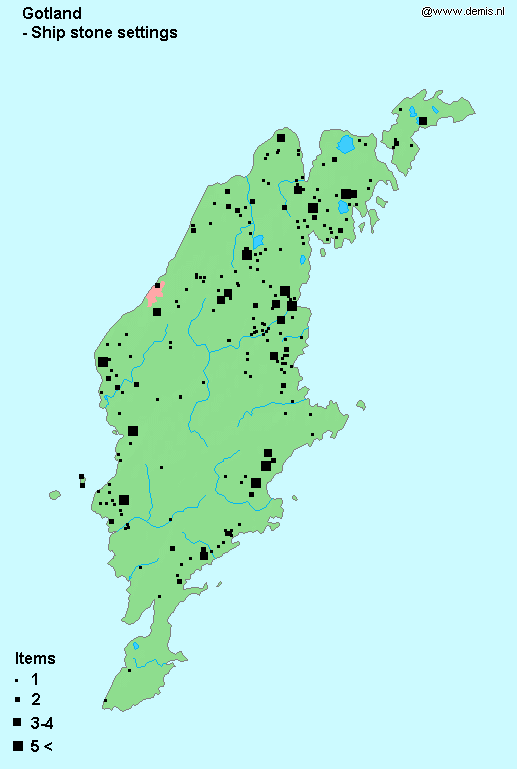
\includegraphics[width=\linewidth]{Clark_Figure01}
	\caption{Distribution of stone ship settings on Gotland, Sweden. 2013.
		{\normalfont\scriptsize \\ \copyright\ by Joakim Wehlin, used with permission.
			%\shortauthor
			% or NAME OF COPYRIGHT HOLDER
	}}
	\label{fig:Clark_Figure01}
\end{figure}

Although archaeological data in Southeast Asia is sparse, ethnographic and ethno-historical information suggests that boat imagery and symbolism plays a major role in rituals associated with rites of passage, life transitions, and death. Furthermore, ships act as the basic social units of family and community, representing communal unity and the ordered social group \parencite[392]{Ballard_2004}.
This is a logical interpretation; to be part of a rowing crew was a social act, and a boat’s crew could be considered a microcosm of the community itself \parencite[46]{Westerdahl_2015}.
In addition, the ship symbol was strongly linked with divinatory, ecstatic, and necromantic ritual in Indonesian and Melanesian shamanic practice; ships could not only be used to ferry souls to the world of the dead, but to communicate with the ancestors \parencite[392]{Ballard_2004}.
Indeed, the association between ships and death in most Austronesian-speaking communities is so strong that the terms for ‘boat’ and ‘coffin’ can be interchangeable \parencites[392]{Ballard_2004}[196]{Manguin_1986}. The connection between ship symbolism and ancestral ritual in Southeast Asia is of particular interest in developing an interpretation of the use and significance of stone ship settings, but what evidence of this relationship can be found in Scandinavian contexts?

To answer this question, the construction of stone ship settings must be considered. Stone ship settings exhibit a great degree of variation in size and proportion (Figs. \ref{fig:Clark_Figure02} and \ref{fig:Clark_Figure03}) and, as funerary markers, their osteological remains and grave goods are just as diverse.
While the average length is 10 meters, their size may range from 2 to 45 meters \parencite[222]{Price_2015}.
A proportional standard also seems not to have been established: smaller stone ship settings possess length: width ratios between 2.5:1 and 4:1, while larger ship settings are far narrower, averaging length: width ratios between 6:1 and 8:1 \parencite[95]{Bradley_2010}.
Some scholars suggest that the ratios of these ship settings may be representative of different types of real ships, including war canoes and transport vessels \parencites{Artursson_2013}{Bradley_2010}[204-205]{Skoglund_2014}. This interpretation implies that the stone ship settings, like their wooden counterparts, may have held different connotations and functions based on size. Warships, which have been compared with large ship settings, are representative of communal unity, working together for a common goal, and social engagement. These ideals align well with rituals involving an entire community, or even multiple communities, coming together as one in a ritualized space. Alternatively, transport vessels, which may have been the inspiration for small ship settings, exist for the purpose of ferrying things from one place to another. In a mortuary context, this symbolism can be understood as a method of transport for the ancestors to and from the world of the dead. While both ship setting sizes may have been used for the purposes of commemorative ritual, the connotations vary slightly from one another.

%FIG 2 and 3
\begin{figure}[!htb]
	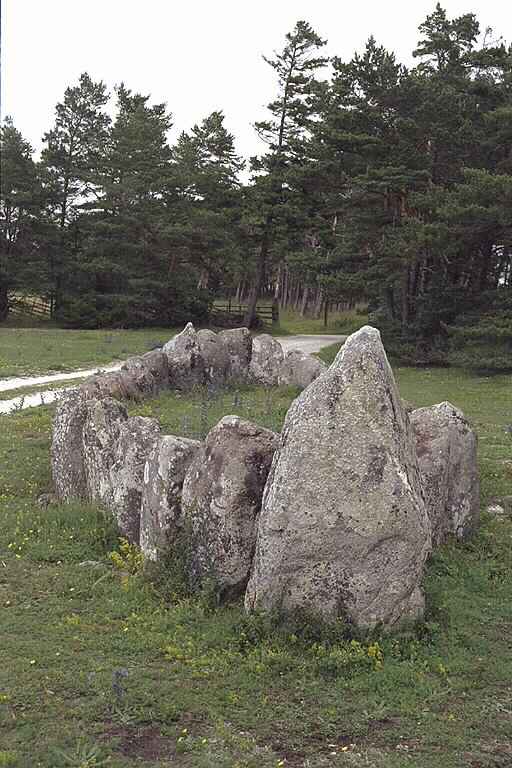
\includegraphics[width=\linewidth]{Clark_Figure02}
	\caption{Stone ship setting in Gnisvärd, Tofta, Gotland, Sweden. 2003.
		{\normalfont\scriptsize \\ \copyright\ by Bengt A. Lundberg and Swedish National Heritage Board, Wikimedia Commons License.
			%\shortauthor
			% or NAME OF COPYRIGHT HOLDER
	}}
	\label{fig:Clark_Figure02}
\end{figure}

\begin{figure}[!htb]
	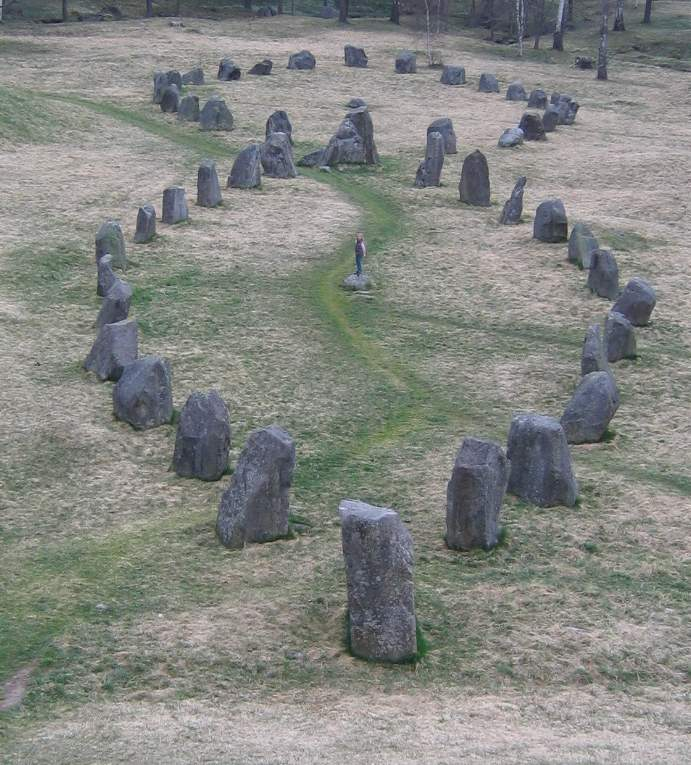
\includegraphics[width=\linewidth]{Clark_Figure03}
	\caption{Two Viking stone ships (burial grounds) at Badekunda, near Västerås, Sweden. 2005.
		{\normalfont\scriptsize \\ \copyright\ Berig, Wikimedia Commons License.
			%\shortauthor
			% or NAME OF COPYRIGHT HOLDER
	}}
	\label{fig:Clark_Figure03}
\end{figure}


A different perspective of the ship’s sizes, and what they may allude to, yields nearly the same results. \textcite{Bradley_2010} notes that the measurements of larger stone ship settings on Gotland also compare favorably with rectangular stone structures believed to be ‘cult houses’ found on the coast of Sweden,
suggesting that perhaps they served similar or identical functions \parencite[97]{Bradley_2010}.
This concept may have a solid archaeological foundation: the remains of fires and feasts have been recovered from within the boundaries of these burial monuments, potentially indicating their purpose as a commemorative place \parencite[261]{Price_2008}.
Yet size distinctions among stone ship settings may have also reflected a difference between memorializing practices; \textcite[97]{Bradley_2010} propose that large stone ship settings may have acted as cult houses for the veneration of important communal ancestors, while smaller settings may have been utilized for the purpose of ancestor veneration at the familial level.

A final element of stone ship setting construction which deserves consideration is the deliberate choice between building the ship’s outline using kerbs or monoliths (Figs. \ref{fig:Clark_Figure04} and \ref{fig:Clark_Figure05}).
In an apt comparison between stone ship settings and contemporary Bronze Age rock art, which depicts ships both with and without crews, \textcite[86--87]{Bradley_2010} theorize that upright stones may not only have had the effect of creating a ship outline – they may also have represented crew members. This effect is compounded when one considers that the monoliths on either side of most Gotlandic ship settings appear to be paired, much like a pair of rowers. Monoliths acting as human representations have ethnographic parallels all over the world, including in Gotlandic folklore. If these stones did indeed represent crew members aboard a ship of the dead, it does not seem implausible to consider that they may have even represented familial or communal ancestors. To be cremated and buried within a metaphorical ship of the dead crewed by one’s ancestors may have been considered a rite of passage in which the dead person left the community of the living to join the community of the dead.

%FIG 4 and 5
\begin{figure}[!htb]
	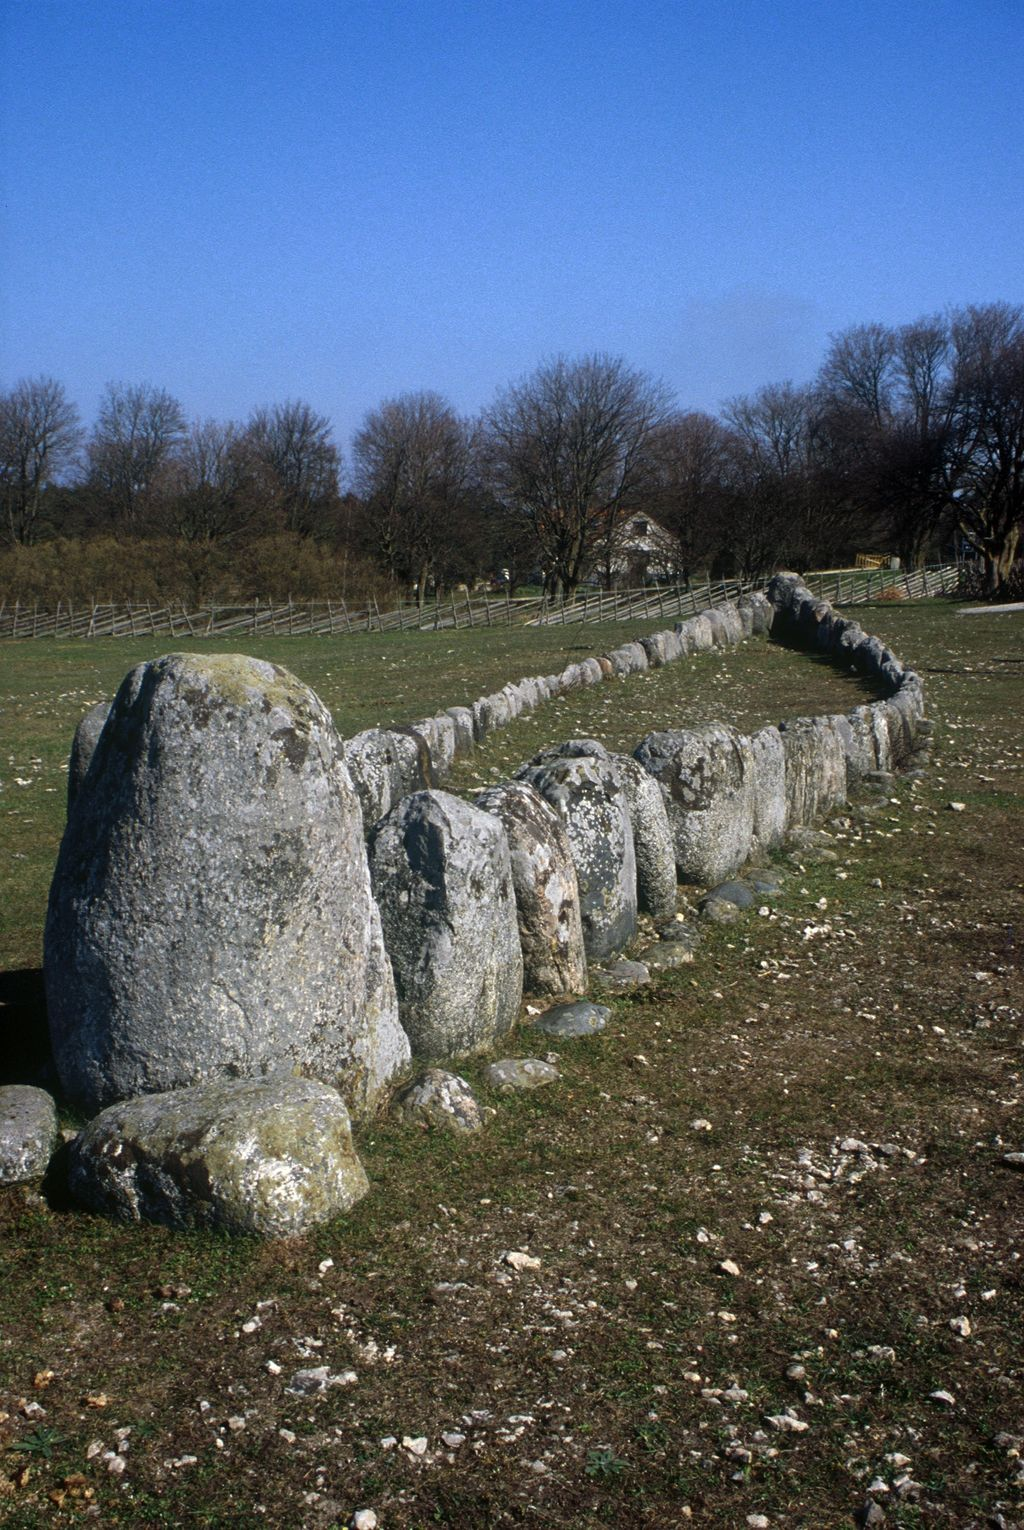
\includegraphics[width=\linewidth]{Clark_Figure04}
	\caption{Stone ship, Gannarve, Gotland, Sweden. 2001.
		{\normalfont\scriptsize \\ \copyright\ by Tyler Bell, Wikimedia Commons License.
			%\shortauthor
			% or NAME OF COPYRIGHT HOLDER
	}}
	\label{fig:Clark_Figure04}
\end{figure}

\begin{figure}[!htb]
	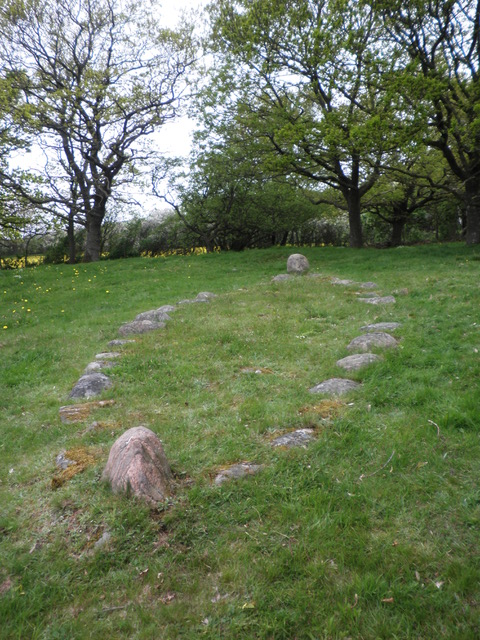
\includegraphics[width=\linewidth]{Clark_Figure05}
	\caption{Stone ship at Tofta högar (RAÄ Number Hov 109:1) in Hov parish, Bjäre hundred, Båstad municipality, Skåne County, Scania, Sweden. 2010.
		{\normalfont\scriptsize \\ \copyright\ ArchEllen, Wikimedia Commons License.
			%\shortauthor
			% or NAME OF COPYRIGHT HOLDER
	}}
	\label{fig:Clark_Figure05}
\end{figure}

However, there is yet another layer to the symbolism of these monoliths. Unlike kerb-constructed ship settings, which Bradley et al. suggests may be “empty” vessels and typically have a clear direction of travel based on the monoliths that mark their prow and stern, the directionality of monolith-constructed ship settings is far more ambiguous. It is possible they may have even been considered to travel in two directions \parencite[88]{Bradley_2010}.
Based upon these interpretations, I posit that stone ship settings were perceived of not only as grave markers, but as ancestral touchpoints – places within the landscape that familial or communal ancestors could return to and depart from aboard a ship that could traverse the boundaries between the worlds of living and dead. Furthermore, some stone ship settings are connected from end to end, lining up one after another \parencite[84]{Bradley_2010}. This suggests that groups of stone ship settings may have had the effect of signaling ancestral relationships and lineages.

Several such examples of Gotlandic stone ship settings which may reference ancestry or familial ties can be found in the Rannarve Klinte parish, in which five definitive stone ship settings and a sixth possible example are found in one place, four of which are in line with one another (Fig. \ref{fig:Clark_Figure06}).
Each ship setting contained the cremated remains of one individual. Excavation of the features revealed that within the second ship setting was a house urn containing burnt bone, sand, and two knives. The fourth ship setting may also have held such a vessel, though prior disturbance of the feature makes this difficult to discern \parencite[7-26]{Gustavsson_2012}. The importance of house urns to an interpretation of ancestor worship will be discussed in the following section.

%FIG 6
\begin{figure}[!htb]
	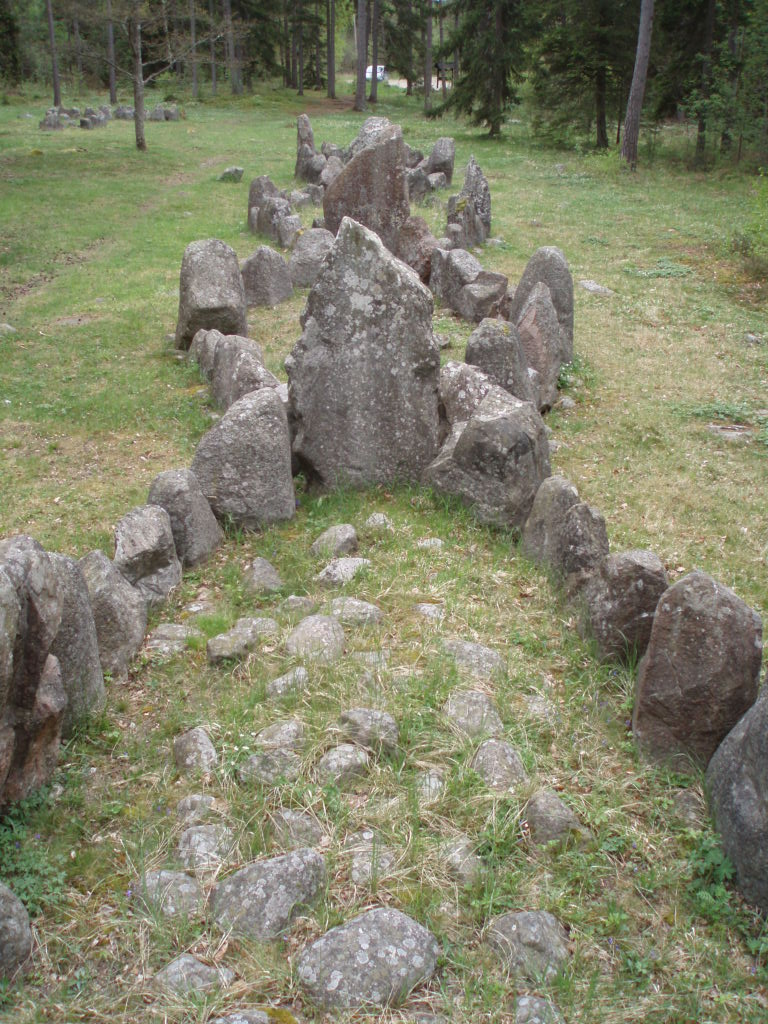
\includegraphics[width=\linewidth]{Clark_Figure06}
	\caption{Stone Ships at Rannarve, near Klintehamn, Gotland, Sweden. 2008.
		{\normalfont\scriptsize \\ \copyright\ BH2008, Wikimedia Commons License.
			%\shortauthor
			% or NAME OF COPYRIGHT HOLDER
	}}
	\label{fig:Clark_Figure06}
\end{figure}

Not far from this row of ship settings is a circular cairn, surrounded by a sizable number of flint pieces. A ceramic urn was found inside a stone cist at the center of the cairn. Inside it, archaeologists found burnt bone, a razor, an awl, and a bronze bar \parencite[7--26]{Gustavsson_2012}.
At first it may seem that this circular structure may be a clear reference to, or continuation of, the Bronze Age association between ships and the sun depicted in rock carvings and on razors from mainland Sweden \parencites{Kaul_1998}[400]{Skoglund_2008}.
However, the contents of the cairn suggest that the structure may have served as a deposition point for offerings made to the ancestors of this family group by their living descendants; even in other mortuary contexts, evidence exists to support the practice of feasting and offering rituals at burial sites long after the burial itself takes place \parencite[261]{Price_2008}. I posit that these ritualized offerings may have been indicative of ancestor veneration and that stone ship settings, like the ship symbol in Southeast Asia, may have been considered access points for the living to commune with the dead.

The Kaupang ship burial in Norway is another example of ancestral referencing and possible veneration within ship-themed funerary contexts (Fig. \ref{fig:Clark_Figure07}).
In this instance, a ship containing a man, two women, and an infant was buried directly on top of a simple one-man grave created decades earlier. The keel of the boat was aligned precisely with the body of the earlier burial, indicating not only that the burial position and location was remembered decades later, but that the individuals within the boat burial sought to replicate or reference these conditions. In this way, the ship burial may be a continuation of, or a reference to, ancestral lineage \parencites[267--268]{Price_2008}{Price_2012b}.

%FIG 7
\begin{figure}[!htb]
	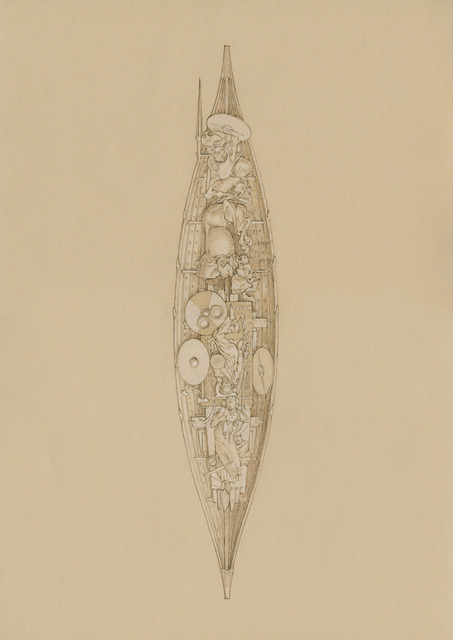
\includegraphics[width=\linewidth]{Clark_Figure07}
	\caption{A boat burial from Kaupang, Norway, early 10th century. Image by Þórhallur Þráinsson.
		{\normalfont\scriptsize \\ \copyright\ Neil Price, used with permission.
			%\shortauthor
			% or NAME OF COPYRIGHT HOLDER
	}}
	\label{fig:Clark_Figure07}
\end{figure}

Returning to Gotland in a later period, one can also find ships represented in registered carvings upon massive stone stelae called picture stones. Dating from \AD 400-1100, picture stones are interpreted as commemorative markers for the dead, as burials have been found at the foot of many of these impressive stones (Fig. \ref{fig:Clark_Figure08}). Because no burials containing actual wooden ships have been found on the island of Gotland, scholars suggest that these picture stones may embody a two-dimensional representation of the continuation of the relationship between ships and death. These intricately decorated stones nearly always depict a ship within the bottom register and heroic, even mythological narratives told in the top registers (Fig. \ref{fig:Clark_Figure09})
\parencite[396--398]{Skoglund_2008}.
This may be a pictorial representation of ancestral veneration and the ‘hero cult’ practice, in which the dead were deified and their identity became conflated with notions of heroism, myth, and legend \parencite[177]{Sundqvist_2015}.
The influence of ancestry and lineage is further manifested upon these stones in the organization of the images themselves. The stories told within the registers reference one another – the top register of one stone can often be found as the bottom register of another stone from the same approximate geographical area. This is suggestive of a familial narrative, telling the story of a lineage in chapters that continue from generation to generation. This not only binds the dead to the living and vice versa, but also deepens the connection between the dead and the land in which they are buried \parencite{Price_2012a}.

%FIG 8
\begin{figure}[!htb]
	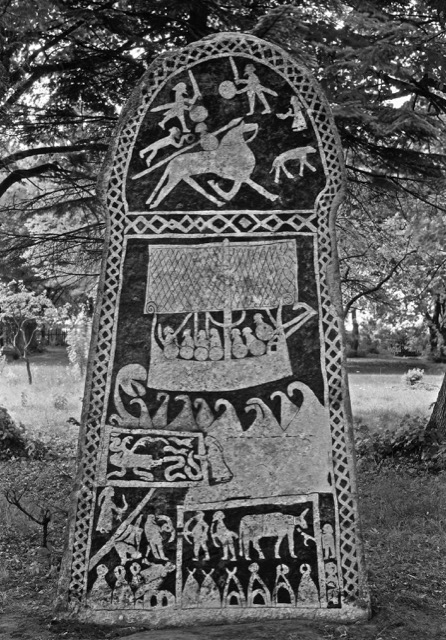
\includegraphics[width=\linewidth]{Clark_Figure08}
	\caption{"The Hunninge stone": Picture Stone nº1 from Hunninge, Gotland. 8th century A.D. The Gotland Museum (Visby).
		{\normalfont\scriptsize \\ \copyright\ Swedish National Heritage Board, Wikimedia Commons License.
			%\shortauthor
			% or NAME OF COPYRIGHT HOLDER
	}}
	\label{fig:Clark_Figure08}
\end{figure}

\begin{figure}[!htb]
	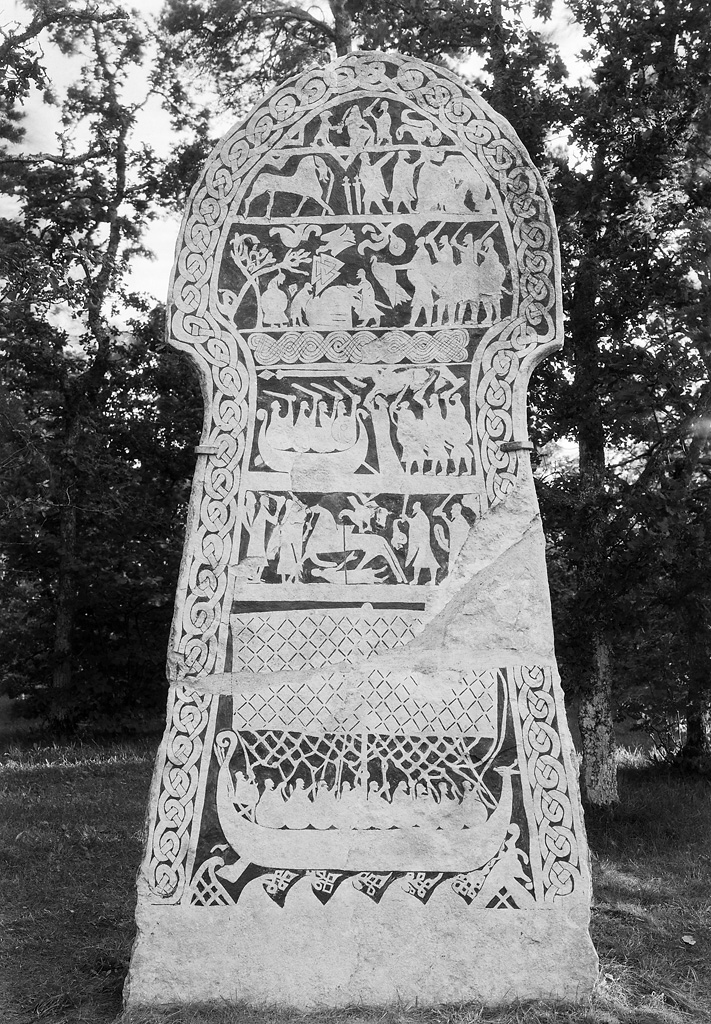
\includegraphics[width=\linewidth]{Clark_Figure09}
	\caption{Viking Age picture stone from Stora Hammars on the island of Gotland, in Bunge Open Air Museum.
		{\normalfont\scriptsize \\ \copyright\ Swedish National Heritage Board, Wikimedia Commons License.
			%\shortauthor
			% or NAME OF COPYRIGHT HOLDER
	}}
	\label{fig:Clark_Figure09}
\end{figure}

\IJSRAsection{Necromancy and Ship-Themed Burials}

As described in the previous section, both burial mounds and cult houses have historically been used for the purposes of ritual, ancestor veneration, and even communication with the dead. Considering the similarities that ship-themed burials share in common with these architectural features, it follows that analogous activities may have taken place at ship burials, stone ship settings, and picture stones – all commemorative markers equal in scale and significance to other monuments constructed to honor the dead. However, if ancestor veneration and ritual is a theme throughout Scandinavian mortuary contexts, what effect can ship symbolism have upon these rituals and perceptions?

If people buried in regular mounds are believed to live there, are people buried within ship-themed burials also considered to reside within their graves? The answer may be more complex than a simple ‘yes’ or ‘no.’ Rather, I suggest that these dead ancestors are believed to undertake great journeys in the afterlife, but that ships and other portals have been provided at the gravesite to forever bind them to the land. Perhaps they are not considered to live there, but are given points of entry so that they might come and go at will or else be summoned by the living. I propose that ancestors who were buried with ships or ship symbols could be summoned back from the land of the dead to speak with or aid their living descendants, travelling between worlds via the sea, a well-known boundary between the lands of the living and dead.

Evidence of necromancy – specifically, waking the dead from their burial mounds to communicate with the living – can be found in runic inscriptions as early as \AD 650-700. Several references to this practice can also be found within the Poetic Edda: \textit{Grogalder} is the story of a son who wakes his mother from the dead to solicit her help.
The \textit{Second Poem of Helgi Hundigsbani} is the tale of a man named Helgi who, after his death and subsequent journey to Valhalla, was summoned to his burial mound to comfort his widow \parencite[171]{Sanmark_2010}.  Based upon this tale, one can conclude that even the dead who ventured to another world, rather than residing in their mounds, could be summoned back to the realm of the living and communicated with. If this is the case, it therefore seems plausible that the practice of calling ancestors back from their seafaring afterlife voyages may have been as common as other forms of ancestor veneration and necromancy.

A more explicit example of the relationship between ship burials, ancestor veneration, and necromancy can be observed from the well-known Oseberg ship burial of Norway (Fig. \ref{fig:Clark_Figure10}).
This burial is the final resting place of two women interpreted variously as two volva sorceresses, a volva and her apprentice, two ostentatious queens, or a queen and her servant \parencite{Ruffoni_2011}.
An array of artifacts including clothing, shoes, cookware, combs, sledges, and tents, as well as the remains of fifteen horses, six dogs, and two cows have been recovered from this funerary context. This richly extravagant ship burial is representative of the relationship between high status burials and ship symbolism throughout the 9th century in Scandinavia \parencite[20--25]{Ruffoni_2011}.
The plentitude of grave goods seems to suggest that the ship and its passengers were well equipped for a long journey into the world of the dead. However, this symbolism is contradicted by another intentional feature of this burial: the ship itself is moored, tied to a massive and immovable boulder \parencite[262]{Price_2008}.

%FIG 10
\begin{figure}[!htb]
	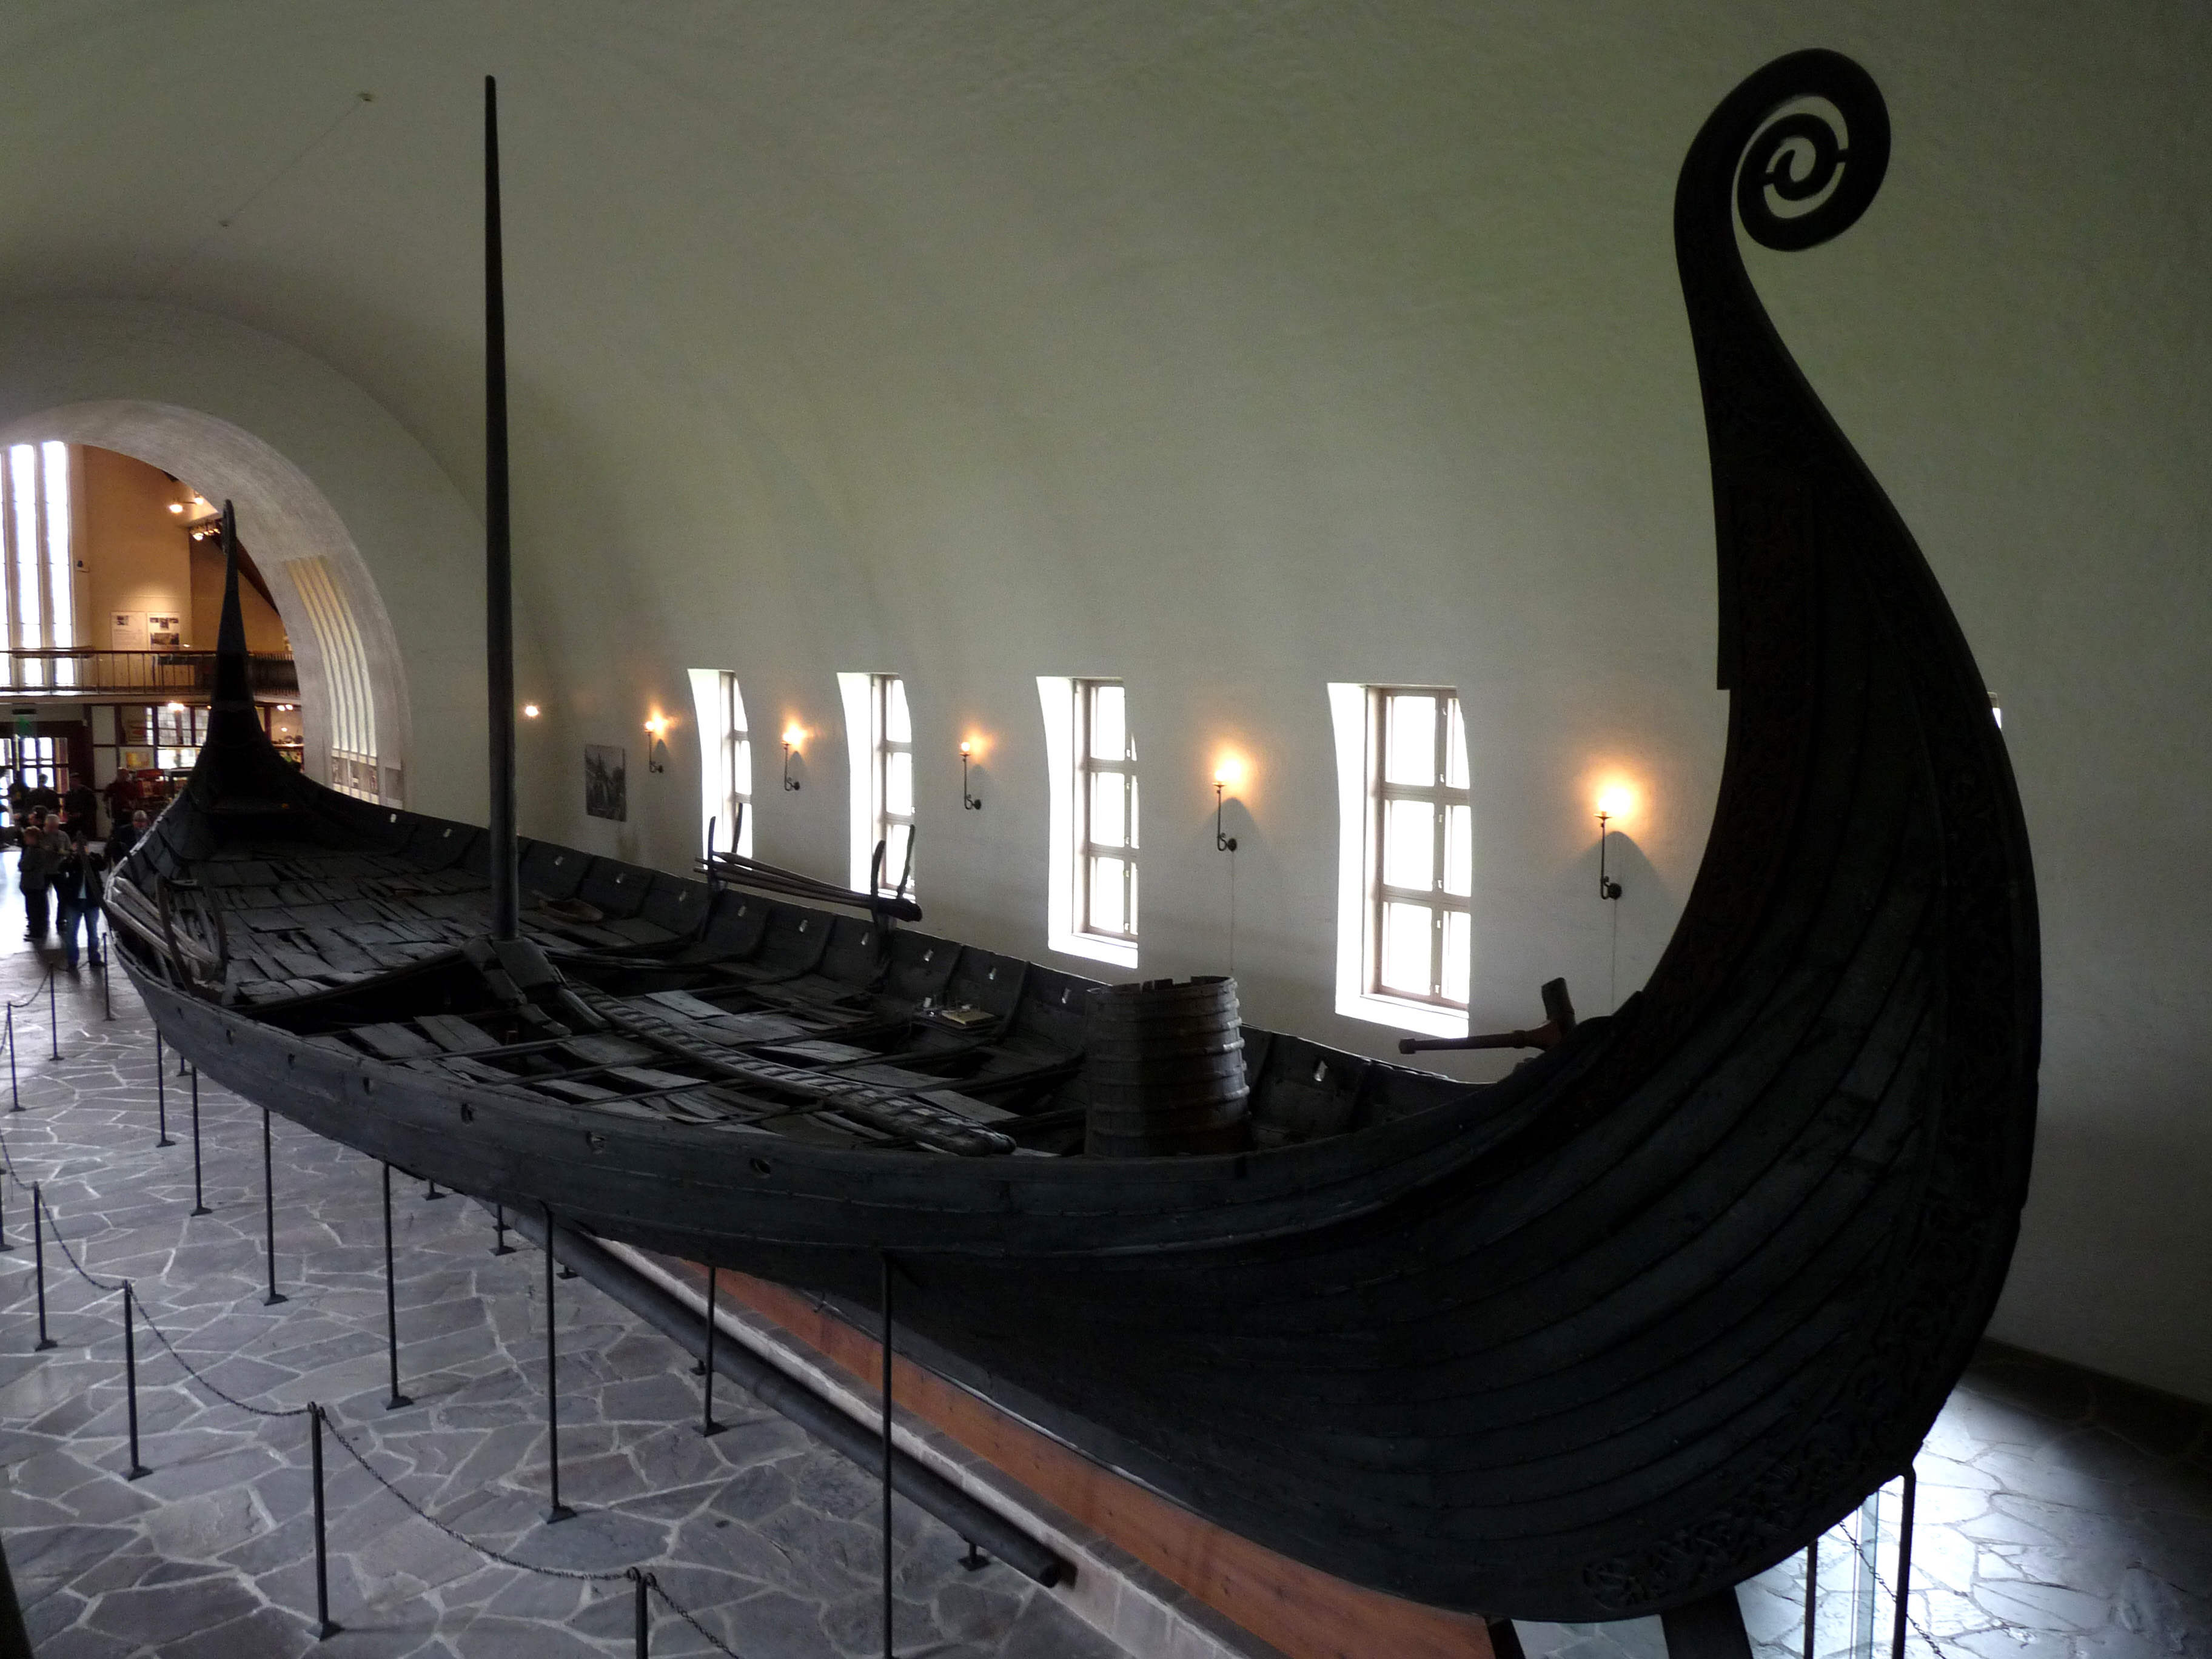
\includegraphics[width=\linewidth]{Clark_Figure10}
	\caption{Oseberg ship in The Viking Ship Museum, Oslo, Norway. 2010.
		{\normalfont\scriptsize \\ \copyright\ Jean Paul Alandry, Wikimedia Commons License.
			%\shortauthor
			% or NAME OF COPYRIGHT HOLDER
	}}
	\label{fig:Clark_Figure10}
\end{figure}

Several theories have been proposed to explain the dichotomous nature of symbolism in this burial. Archaeologist Anne Stine Ingstad posited that the act of fastening the ship to a boulder would have ensured that the Oseberg women would remain in the mound that covered their ship burial to guarantee prosperity and fertility to the land they surveyed. Norwegian archaeologist Brit Solli offered another tantalizing interpretation. Presuming that one of the women in the burial was a volva sorceress, Solli proposed that this intentional mooring was indicative of necromantic practices. Specifically, this burial feature was designed to guide the woman’s soul back to her mound, referred to as her “dwelling,” after being summoned to perform some magical task by the living \parencite[33]{Ruffoni_2011}.
A final interpretation theorized that the mooring of the ship burial does not discredit the implication of posthumous travel suggested by the vessel; rather, this act may indicate that the women dwelled in the burial mound only temporarily, and could decide for themselves when to depart from this world aboard the ship within which they were buried \parencite[216--217]{Bill_2016}.
The Oseberg burial was broken into and raided over a century later; archaeologist Jan Bill suggests that this act was meant to rob these high status individuals of their power to legitimate other rulers in the area. If this is the case, it seems plausible that the two women were believed to reside within the mound and possess agency and power over the living for at least a hundred years after their burial \parencite[218]{Bill_2016}.
Particularly relevant to my interpretation is the concept that “the ship is lying ready for departure, but is still connected to the imaginary coast \parencite[212]{Bill_2016}.” It is through this metaphorical connection that the dead remained bound simultaneously to their descendants, to the land, and to the afterlife.

Symbolism suggestive of both travel and domesticity is reflected in mortuary ships and the mounds within which they are buried, as well as stone ship settings and the house urns found within them. Indeed, house urns found in stone ship settings may have had a similar effect to the mooring evident at Oseberg. Archaeologists and historians are still in disagreement as to whether house urns may have represented real houses – on Gotland, abroad, or as a spiritual 'house' in the afterlife \parencite[80]{Runesson_2010}. At first glance, it seems possible that these metaphorical houses may have been integrated in funerary monumentality with the express intent of providing a home for the dead to dwell in after death. However, much like other mortuary settings, I suggest that these miniature houses were meant to be used as a touchstone – a point within the landscape to which the dead could always return, either from their travels in the afterlife or after being summoned by the living via necromancy. This interpretation seems more likely in the context of a ship burial; the juxtaposition of symbolism suggestive of both travel and sedentariness insinuates that both aspects of life were crucial in the afterlife.

Similar symbolism may also be apparent in examples of stone ship settings on the Swedish mainland. These ship-shaped monuments were typically paired with small, rectangular stone settings whose proportions mimic Late Bronze Age domestic buildings, albeit on a miniature scale. It has been suggested that the pairing of ship and house symbolism was meant to represent the sea and the land \parencite[93]{Bradley_2010}. However, considering this from the perspective of mortuary behavior and cosmological ideologies, it does not seem a stretch to perceive of the dichotomy exemplified by these structures as representative of the ancestors’ travels between the worlds of living and dead. The ship, clearly linked with the concepts of travel, is offset by the ideological representation of a home to which the dead can also return.

The practice of ancestor veneration and communication may also apply to the picture stones of Gotland. Scholars have observed that the shape of these massive memorial stones for the dead strongly correlates with the shape of stave church doors \parencite[195-196]{Eriksen_2013}.
The parallelism of these two architectural features may indicate that these monuments were believed to be access points – doors – to the realm of the dead. Indeed, verses from the Poetic Edda allude to doors as portals used for travel to the death realm; the gateway to Hel is even described as a door. Other passages from the Poetic Edda explicitly reference the relationship between doors and necromancy. In one, Odin journeys to the death realm to solicit the advice of a dead volva, who is buried “east of the door,” and whom he awakens with sorcery. Another poem describes a son waking his sorceress mother from the grave, saying, “Wake three, Groa, wake, mother good, at the doors of the dead I call thee \parencite[191-194]{Eriksen_2013}.”

The relationship between ships and doors is further elucidated in Ibn Fadlan’s firsthand account of a chieftain’s ship burial, which provides a detailed characterization of the use of doors in funerary and necromantic ritual, including those mortuary contexts grounded in ship symbolism. Fadlan described how a slave girl, who volunteered to be sacrificed for her dead master, is raised above a ritually crafted “door”; the girl, upon peering over the top of the door, exclaims, “Behold, I see my father and my mother... Behold, I see all of my dead kindred... Behold, I see my master, seated in Paradise \parencite[17-18]{Montgomery_2000}.”
Based upon this literary evidence, it seems that doors and door-shaped picture stones in mortuary contexts were explicitly used as a way to see, travel to, or communicate with the afterlife \parencite{Price_2012a}. For the purposes of my argument, Ibn Fadlan’s account has the added benefit of merging the ritual use of doors with both ship burials and necromancy, substantiating the claim that the dead interred in ship-themed burials were actively venerated and communicated with. The relationship between doors and ships found in Ibn Fadlan’s narrative is mirrored in the form and design of Gotlandic picture stones, the bottom register of which always features a ship. It is possible that ship and door symbolism worked in conjunction with one another. Perhaps ships were considered the vessel within which the dead could travel between the living and dead worlds, while doors and door-shaped picture stones served as portals through which the dead and living could communicate.

Although moored mound-dwelling ships, stone ship settings containing house urns, and door-shaped picture stones may at first seem to convey various underlying meanings, I argue that the implied permanence of these burial monuments as homes or as access points to the world of the living provided the dead a place within the landscape to return to when summoned by their descendants. In this way, their souls could not lose their way or become trapped during their journey, nor could they be fully separated from their land or lineage.

The deliberate liminality in the placement and construction of ship-themed burials is a final and crucial component in the interpretation of ancestor veneration and necromancy in association with mortuary ship symbolism. The intentional positioning of Gotlandic picture stones along property lines is evocative of cosmological boundaries as well as travel between the worlds of living and dead. This symbolism is compounded by the shape of these monuments; doors are, in and of themselves, suggestive of travel and transition, and these mortuary doors are representative of points of entry from one world to another \parencites[195--196]{Eriksen_2013}{Price_2012a}.
Liminality is also apparent in the placement and construction of stone ship settings. All recorded discoveries of these monuments have been situated near water. Though this may be a clear parallel to the real objects they imitated \parencite[47]{Wallin_2010},
it is imperative to consider that bodies of water were also cosmologically liminal places, demarcating the periphery between the lands of living and dead \parencites[388]{Ballard_2004}{Helskog_1999}[91]{Wehlin_2010}.
Curiously, the construction of monolithic stone ship settings also displays a certain ambiguity in the directionality of travel. It is possible that these monuments were believed to travel in both directions \parencite[89]{Bradley_2010}, eliciting the concept of afterlife mobility in terms of both departure and return. I suggest that the placement of these burial features in intermediary points within the landscape was a deliberate aspect of ship-themed burial ritual that allowed the dead to travel back and forth between the worlds with ease.

\IJSRAsection{Conclusion}

While mortuary ships are typically understood as vessels of transportation from the world of the living to the world of the dead, I believe this interpretation is far too simple. The symbolism contained within ship-themed burials is incredibly complex, but it is clear that these burials fit firmly within a mortuary tradition that honored and communicated with dead ancestors. While individuals buried in mounds were often believed to dwell within the land, it seems that those whose burials contained ship symbolism were believed to be capable both of journeying to another world and of returning when called upon via necromancy. Elements of their construction frequently evoke both travel and domesticity, departure and return, while simultaneously referencing ancestral lineage. The liminal position and construction of burials containing ship symbolism is suggestive, too, of transition and travel between worlds. The ship these ancestors were buried with enabled them to cross the proverbial sea, the cosmological boundary between the worlds of living and dead. However, the evidence presented in this analysis suggests that even the dead interred within ship-themed burials were still anchored to the world of the living. Sometimes the connection between the worlds was manifested in obvious physical ways, like the mooring of the Oseberg ship and the house urns found within stone ship settings. Alternately, the link between the ancestors and the world of the living may have been maintained through cultural perspectives and interactions with the dead. Evidence of this practice can be found in the remains of commemorative feasts and rituals that took place within Gotlandic stone ship settings, or in literature describing the necromantic practices employed by Old Norse peoples to wake their ancestors from their graves, including those in ship burial mounds and burials beneath picture stones.

Although the evidence presented within this paper addresses the practice of ancestor veneration and necromancy within the context of ship-themed burials, many questions remain for future research. Why were certain ancestors chosen to experience an afterlife of travel within the cosmic sea, while others remained within their mounds to sing and watch over the land? Did early Scandinavian people believe that ancestors buried with ship symbols could access sacred knowledge unattainable to those who dwelled eternally in their mounds? Was there an archaeologically observable difference between the commemorative and necromantic practices of burial mounds and ship-themed burials? Some of these questions are quite cerebral in nature and thus, their answers may elude us. This does not mean that we should not make the attempt to address these questions, however. It is my hope that in the future, interpretations of mortuary ship symbolism will finally move beyond the simple and much-studied notion of posthumous travel and will instead endeavor to further explore the relationship between identity, cosmology, and ship symbolism.


\IJSRAseparator


\IJSRAclosing%<---- don’t change this!
